\documentclass{math}

\usepackage{tikz}
\usetikzlibrary{arrows.meta}

\title{Differential Equations}
\author{Alvin Lin}
\date{January 2018 - May 2018}

\begin{document}

\maketitle

\section*{Laplace Transforms}
Let \( f \) be a function defined on \( [0,\infty) \). The Laplace transform
of \( f \), \( \laplace{f(s)} \), is a function \( F(s) \), where \( s \)
is the new variable. The domain of \( \laplace{f} \), or \( F(s) \), is all
values of \( s \) for which the following converges:
\[ \laplace{f} = \int_{0}^{\infty}\e^{-st}f(t)\diff{t} \]
Recall the following:
\[ \int_{0}^{\infty}g(t)\diff{t} = \lim_{N\to\infty}\int_{0}^{N}g(t)\diff{t} \]
If this limit exists, it converges. Otherwise, it diverges.

\subsubsection*{Example}
Find \( \laplace{f(t)} \) where \( f(t) = 1 \).
\begin{align*}
  \laplace{1} &= \int_{0}^{\infty}\e^{-st}\diff{t} \\
  &= \lim_{N\to\infty}\int_{0}^{\infty}\e^{-st}\diff{t} \\
  &= \lim_{N\to\infty}\bigg[-\frac{1}{s}\e^{-st}\bigg]_{0}^{N} \\
  &= \lim_{N\to\infty}\bigg[-\frac{1}{\e^{sN}}-\bigg(-\frac{1}{s}\bigg)\bigg] \\
  &= \frac{1}{s}, \quad s > 0
\end{align*}
Additional fact: \( \laplace{0} = 0 \).

\subsubsection*{Example}
Find \( \laplace{\e^{at}} \) where \( a \) is real.
\begin{align*}
  f(t) &= \e^{at} \\
  \laplace{\e^{at}} &= \int_{0}^{\infty}\e^{-st}\e^{at}\diff{t} \\
  &= \int_{0}^{\infty}\e^{-(s-a)t}\diff{t} \\
  &= \lim_{N\to\infty}\int_{0}^{N}\e^{-(s-a)t}\diff{t} \\
  &= \lim_{N\to\infty}\bigg[-\frac{1}{s-a}\e^{-(s-a)t}\bigg]_{0}^{N} \\
  &= \lim_{N\to\infty}\bigg[-\frac{1}{s-a}\e^{-(s-a)N}-
    \bigg(-\frac{1}{s-a}\bigg)\bigg] \\
  &= \lim_{N\to\infty}-\frac{1}{s-a}\e^{-(s-a)N}+\frac{1}{s-a} \\
  &= \frac{1}{s-a}, \quad s-a > 0 \\
  &= \frac{1}{s-a}, \quad s>a \\
  \laplace{\e^{2t}} &= \frac{1}{s-2} \\
  \laplace{\e^{-2t}} &= \frac{1}{s+2}
\end{align*}

\subsubsection*{Example}
Find \( \laplace{t} \).
\begin{align*}
  f(t) &= t \\
  \laplace{t} &= \int_{0}^{\infty}t\e^{-st}\diff{t} \\
  &= \lim_{N\to\infty}\int_{0}^{N}t\e^{-st}\diff{t} \\
\end{align*}
\begin{align*}
  &= \lim_{N\to\infty}\bigg[-\frac{1}{s}\e^{-st}t\bigg]_{0}^{N}-
    \int_{0}^{N}-\frac{1}{s}\e^{-st}\diff{t} \\
  &= \lim_{N\to\infty}\bigg[
    -\frac{1}{s}\e^{-st}t+\frac{1}{s}(-\frac{1}{s}\e^{-st})\bigg]_{0}^{N}
  &= \lim_{N\to\infty}\bigg[
    (-\frac{1}{s}\e^{-sN}N)+(-\frac{1}{s^2}\e^{-sN}-\frac{1}{s^2})\bigg] \\
  &= \frac{1}{s^2}, \quad s>0
\end{align*}
As a general rule, for \( f(t) = t^n \) where \( n \) is a non-negative integer:
\begin{align*}
  \laplace{t^n} &= \frac{n!}{s^{n+1}} \\
  \laplace{t^3} &= \frac{3!}{s^{3+1}} = \frac{6}{s^4}
\end{align*}
Additionally, for sines and cosines:
\begin{align*}
  \laplace{\sin(bt)} &= \frac{b}{s^2+b^2}, \quad s>0,b\ne0 \\
  \laplace{\cos(bt)} &= \frac{s}{s^2+b^2}, \quad s>0,b\ne0 \\
  \laplace{\sin(\sqrt{2}t)} &= \frac{\sqrt{2}}{s^2+2} \\
  \laplace{\cos(\sqrt{2}t)} &= \frac{s}{s^2+2}
\end{align*}

\subsection*{Property of Linearity}
Given \( f(t),g(t) \) and \( k \) a constant:
\begin{enumerate}
  \item \( \laplace{f(t)\pm g(t)} = \laplace{f(t)}\pm\laplace{g(t)} \)
  \item \( \laplace{kf(t)} = k\laplace{f(t)} \)
\end{enumerate}

\subsubsection*{Example}
\[ \laplace{7+5\e^{-7t}-7\sin(3t)+7t^2+5\cos(7t)} \]
\begin{align*}
  &= \laplace{7}+\laplace{5\e^{-7t}}-\laplace{7\sin(3t)}+\laplace{7t^2}+
    \laplace{5\cos(7t)} \\
  &= 7\laplace{1}+5\laplace{\e^{-7t}}-7\laplace{\sin(3t)}+7\laplace{t^2}+
    5\laplace{\cos(7t)} \\
  &= \frac{7}{s}+\frac{5}{s+7}-\frac{(7)(3)}{s^2+9}+\frac{(7)(2!)}{s^3}+
    \frac{5s}{s^2+49}, \quad s>0
\end{align*}
Note that each term has a different condition for \( s \), so we need to take
the intersection of the conditions.

\subsection*{Existence of the Transform}
Consider a piecewise continuous function \( f \) over \( [a,b] \). \( f \) has
a finite number of jump discontinuities.
\begin{center}
  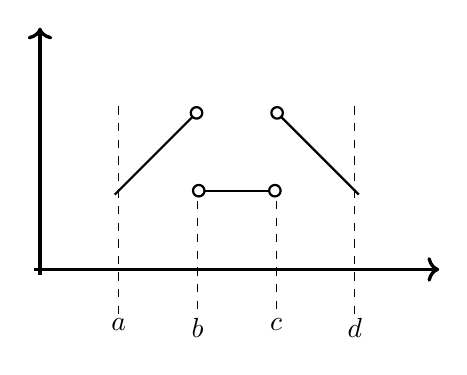
\begin{tikzpicture}[shorten >=-2pt,shorten <=-2pt]
    \draw[->,very thick] (0,0) -- (5,0);
    \draw[->,very thick] (0,0) -- (0,3);
    \draw[dashed] (1,2) -- (1,-0.5) node[below] {\( a \)};
    \draw[thick,-{Circle[open]}] (1,1) -- (2,2);
    \draw[dashed] (2,0.8) -- (2,-0.5) node[below] {\( b \)};
    \draw[thick,{Circle[open]}-{Circle[open]}] (2,1) -- (3,1);
    \draw[dashed] (3,0.8) -- (3,-0.5) node[below] {\( c \)};
    \draw[thick,{Circle[open]}-] (3,2) -- (4,1);
    \draw[dashed] (4,2) -- (4,-0.5) node[below] {\( d \)};
  \end{tikzpicture}
\end{center}
We can extend over \( [0,\infty) \). A function \( f \) is piecewise continuous
over \( [0,\infty) \) if \( f \) is piecewise continuous over \( [0,N] \) for
all \( N > 0 \).
\[ \int_{a}^{d}f(t) = \int_{a}^{b}f(t)+\int_{b}^{c}f(t)+\int_{c}^{d}f(t) \]

\subsubsection*{Exponential Order \( \alpha \)}
A function \( f \) is of exponential order \( \alpha \) if there exists
positive constants \( M \) and \( T \) such that \( |f(t)|\le M\e^{\alpha t} \)
for all \( t > T \). For example:
\begin{align*}
  f(t) &= \e^{2t}\sin(t) \\
  |\e^{2t}\sin(t)| &= \e^{2t}|\sin(2t)| \le
    M\e^{2t} = \e^{2t} \text{ for all } T \\
  |\sin(2t)| &\le 1
\end{align*}
\( f(t) \) is of exponential order \( \alpha = 2 \).

\subsubsection*{Conditions for Existence of the Laplace Transform}
\begin{enumerate}
  \item If \( f(t) \) is piecewise continuous and of exponential order
  \( \alpha \), then the Laplace transform \( \laplace{f(t)} \) exists for
  \( s>a \).
  \item We need to know that
  \[ \laplace{f(t)} = \int_{0}^{\infty}\e^{-st}f(t)\diff{t} \]
  converges for \( s>a \). We can rewrite it as
  \[ \int_{0}^{\infty}\e^{-st}f(t)\diff{t} = \int_{0}^{T}\e^{-st}f(t)\diff{t}+
    \int_{T}^{\infty}\e^{-st}f(t)\diff{t} \]
  where we have \( |f(t)|\le M\e^{\alpha t} \) for all \( t > T \). By
  continuity, \( \int_{0}^{T}\e^{-st}f(t)\diff{t} \) exists, so we only need to
  consider \( \int_{T}^{\infty}\e^{-st}f(t)\diff{t} \).
  \begin{align*}
    \int_{T}^{\infty}\e^{-st}f(t)\diff{t} &=
      \lim_{N\to\infty}\int_{T}^{N}\e^{-st}f(t)\diff{t} \\
    &\le \lim_{N\to\infty}\int_{T}^{N}M\e^{-st}\e^{\alpha t}\diff{t} \\
    &= \lim_{N\to\infty}M\int_{T}^{N}\e^{-(s-\alpha)t}\diff{t} \\
    &= \lim_{N\to\infty}M\bigg[
      -\frac{1}{s-\alpha}\e^{-(s-\alpha)t}\bigg]_{T}^{N} \\
    &= \lim_{N\to\infty}M\bigg[-\frac{1}{s-\alpha}\e^{-(s-\alpha)N}-
      (-\frac{1}{s-\alpha}\e^{-(s-\alpha)T})\bigg] \\
    &= \frac{M}{s-\alpha}\e^{-(s-\alpha)T} < \infty
  \end{align*}
\end{enumerate}
Since \( M \) and \( T \) are positive constants, this integral converges by
the comparison test for improper integrals.

\subsection*{Properties of the Transform}
\begin{itemize}
  \item Translation in \( s \): If the Laplace transform \( \laplace{f(t)} =
  F(s) \) exists, then \( \laplace{\e^{\alpha t}f(t)} = F(s-a) \).
  \( \e^{\alpha t} \) indicates a translation in the \( s \) domain, where we
  replace \( s \) by \( s-a \) in the transform of \( f(t) \). For example:
  \begin{align*}
    \laplace{\e^{2t}\sin(2t)} & \quad \alpha = 2 \\
    \laplace{\sin(2t)} &= \frac{2}{s^2+4} \\
    \laplace{\e^{2t}\sin(2t)} &= \frac{2}{(s-2)^2+4}
  \end{align*}
  Another example:
  \begin{align*}
    \laplace{\e^{-2t}\cos(2t)} & \quad \alpha = -2 \\
    \laplace{\cos(2t)} &= \frac{s}{s^2+4} \\
    \laplace{\e^{-2t}\cos(2t)} &= \frac{s+2}{(s+2)^2+4}
  \end{align*}
\end{itemize}

\subsection*{The Laplace Transform of the Derivative}
Let \( f \) be continuous on \( [0,\infty) \) and \( f' \) be piecewise
continuous on \( [0,\infty) \) and both are of exponential order \( \alpha \).
\begin{align*}
  \laplace{f'(t)} &= \int_{0}^{\infty}\e^{-st}f'(t)\diff{t} \\
  &= \lim_{N\to\infty}\int_{0}^{N}\e^{-st}f'(t)\diff{t} \\
  u &= \e^{-st} \quad\quad\quad\quad \diff{v} = f'(t)\diff{t} \\
  \diff{u} &= -s\e^{-st}\diff{t} \quad\quad v = f(t) \\
  &= \lim_{N\to\infty}\bigg[\e^{-st}f(t)\bigg]_{0}^{N}+
    \lim_{N\to\infty}s\int_{0}^{N}\e^{-st}f(t)\diff{t} \\
  &= -f(0)+sF(s) \\
  &= sF(s)-f(0)
\end{align*}
In summary:
\begin{align*}
  \laplace{y'} &= sY(s)-y(0) \\
  \laplace{y''} &= s^2Y(s)-sy(0)-y'(0)
\end{align*}

\subsection*{Derivatives of the Laplace Transform}
Let \( F(S) = \laplace{f(t)} \). Then for \( s>a \):
\[ \laplace{t^nf(t)} = (-1)^n\ddiff{^nF}{s^n} \]
For example:
\begin{align*}
  \laplace{t\sin(t)} & \quad n = 1 \quad f(t) = \sin(t) \\
  \laplace{\sin(t)} &= \frac{1}{s^2+1} = F(s) \\
  \ddiff{F}{s} &= \ddiff{}{s}\bigg[\frac{1}{s^2+1}\bigg] \\
  &= \frac{(s^2+1)(0)-1(2s)}{(s^2+1)^2} \\
  &= \frac{-2s}{(s^2+1)^2} \\
  \laplace{t\sin(t)} &= (-1)^1\frac{-2s}{(s^2+1)^2} = \frac{2s}{(s^2+1)^2}
\end{align*}
Another example:
\begin{align*}
  \laplace{t\e^{-2t}\sin(3t)} & \quad n = 1 \quad f(t) = \e^{-2t}\sin(3t) \\
  F(s) &= \laplace{\e^{-2t}\sin(3t)} \\
  \laplace{\sin(3t)} &= \frac{3}{s^2+9} \\
  \laplace{\e^{-2t}\sin(3t)} &= \frac{3}{(s+2)^2+9} = F(s) \\
  \ddiff{}{s}F(s) &= \frac{0-(3(2(s+2)))}{((s+2)^2+9)^2} \\
  &= \frac{-6(s+2)}{((s+2)^2+9)^2} \\
  \laplace{t\e^{-2t}\sin(3t)} &= (-1)^1\frac{-6(s+2)}{((s+2)^2+9)^2} \\
  &= \frac{6(s+2)}{((s+2)^2+9)^2} \\
\end{align*}

\subsection*{Inverse Laplace Transforms}
The Laplace transform maps a function \( f(t) \) to a function \( F(s) =
\laplace{f(t)} \). The transform has an inverse denoted by:
\[ \ilaplace{f(t)} = f(t) \]
Consider the following initial value problem:
\[ y''-y = -t \quad y(0) = 0 \quad y'(0) = 1 \]
If we apply the Laplace transform to the entire equation:
\begin{align*}
  \laplace{y''-y} &= \laplace{-t} \\
  \laplace{y''}-\laplace{y} &= -\laplace{t} \\
  s^2Y(s)-(s)y(0)-y'(0)-Y(s) &= -\frac{1}{s^2} \\
  (s^2-1)Y(s) &= -\frac{1}{s^2}+1 \\
  &= \frac{-1+s^2}{s^2} \\
  Y(s) &= \frac{1}{s^2} \\
  \ilaplace{Y(s)} &= \ilaplace{\frac{1}{s^2}} \\
  t &= y(t)
\end{align*}
Given \( F(s) \), if there exists a function \( f(t) \) that is continuous on
\( [0,\infty) \) where \( \laplace{f(t)} = F(s) \), \( f(t) \) is the inverse
of \( F(s) \). The inverse Laplace transform is a linear operator. Given
\( F_1(s), F_2(s) \) and \( k \) a constant, the properties of linearity apply:
\begin{enumerate}
  \item \( \ilaplace{F_1(s)\pm F_2(s)} =
  \ilaplace{F_1(s)}\pm\ilaplace{F_2(s)} \)
  \item \( \ilaplace{kF_1(s)}\pm = k\ilaplace{F_1} \)
\end{enumerate}

\subsubsection*{Example}
\begin{align*}
  \ilaplace{\frac{3}{s^2+9}} &= \ilaplace{\frac{3}{s^2+3^2}} \\
  &= \sin(3t) \\
  \ilaplace{\frac{s-2}{(s-2)^2+4}} &= \e^{2t}\cos(2t) \\
  \ilaplace{\frac{1}{s-6}} &= \e^{6t}
\end{align*}

\subsubsection*{Review of Partial Fraction Decomposition: Case 1}
Suppose we have \( f(x) = \frac{P(x)}{Q(x)} \) and the degree
of \( P \) is less than the degree of \( Q \).
\[ \frac{P(x)}{Q(x)} =
  \frac{P}{(a_1x+b_1)(a_2x+b_2)\cdot\cdot\cdot(a_nx+b_n)} \]
We have \( n \) distinct linear factors that are irreducible, which we can
rewrite as:
\[ \frac{P(x)}{Q(x)} =
  \frac{A_1}{a_1x+b_1}+\frac{A_2}{a_2x+b_2}+\dots+\frac{A_n}{a_nx+b_n} \]
where all \( A_i \)'s are constants. For example:
\begin{align*}
  \frac{x+4}{x^2+3x+2} &= \frac{x+4}{(x+1)(x+2)} \\
  &= \frac{A}{x+1}+\frac{B}{x+2} = \frac{A(x+2)+B(x+1)}{(x+1)(x+2)} \\
  x+4 &= A(x+2)+B(x+1) \\
  Let: x &= -2 \\
  -2+4 &= -B \quad B = -2 \\
  Let: x &= -1 \\
  A &= 3 \\
\end{align*}
This can be applied to inverse Laplace transforms:
\[ \ilaplace{\frac{3s+2}{s^2+s-2}} \]
\begin{align*}
  \frac{3s+2}{s^2+s-2} &= \frac{3s+2}{(s+2)(s-1)} \\
  &= \frac{A}{s+2}+\frac{B}{s-1} \\
  &= \frac{A(s-1)+B(s+2)}{(s+2)(s-1)} \\
  3s+2 &= A(s-1)+B(s+2) \\
  Let: s &= 1 \quad 5 = 3B \quad B = \frac{5}{3} \\
  Let: s &= -2 \quad A = \frac{4}{3}
\end{align*}
\begin{align*}
  \ilaplace{\frac{3s+2}{s^2+s-2}} &=
    \ilaplace{\frac{4}{3}\frac{1}{s-1}+\ilaplace{\frac{5}{3}\frac{1}{s+2}}} \\
  &= \frac{4}{3}\ilaplace{\frac{1}{s-1}}+\frac{5}{3}\ilaplace{\frac{1}{s+2}} \\
  &= \frac{4}{3}\e^t+\frac{5}{3}\e^{-2t}
\end{align*}

\subsubsection*{Review of Partial Fraction Decomposition: Case 2}
In this case, we can have \( n \) repeated linear factors:
\[ f(x) = \frac{P(x)}{Q(x)} = \frac{P(x)}{(a_1x+b_1)^n} = \frac{A_1}{a_1x+b_1}+
  \frac{A_2}{(a_1x+b_1)^2}+\dots+\frac{A_n}{(a_1x+b_1)^n} \]
For example:
\[ \ilaplace{\frac{s^2+9s+2}{(s-2)^2(s+3)}} \]
\begin{align*}
  \frac{A}{s+3}+\frac{B}{s-1}+\frac{C}{(s-1)^2}
    &= \frac{A(s-1)^2+B(s+3)(s-1)+C(s+3)}{(s-1)^2(s+3)} \\
  s^2+9s+2 &= A(s-1)^2+B(s+3)(s-1)+C(s+3) \\
  Let: s &= 1 \\
  1+9+2 &= 4C \quad 4C = 12 \quad C = 3 \\
  Let: s &= -3 \\
  9-27+2 &= 16A \quad A = -1 \\
  Let: S &= 0 \\
  2 &= -1-3B+3C \quad B = 2 \\
  \ilaplace{\frac{s^2+9s+2}{(s-2)^2(s+3)}} &= \ilaplace{\frac{-1}{s+3}+
    \frac{2}{s-1}+\frac{3}{(s-1)^2}} \\
  &= -\ilaplace{\frac{1}{s+3}}+2\ilaplace{\frac{1}{s-1}}+
    3\ilaplace{\frac{1}{(s-1)^2}} \\
  &= -\e^{-3t}+2\e^t+3t\e^t
\end{align*}

\subsubsection*{Review of Partial Fraction Decomposition: Case 3}
In this case, we have \( n \) irreducible distinct quadratics:
\begin{align*}
  \frac{P(x)}{Q(x)} &=
    \frac{P(x)}{(a_1x^2+b_1x+c)\cdot\cdot\cdot(a_nx^2+b_nx+c_n)} \\
  &= \frac{A_1x+B_1}{a_1x^2+b_1x+c_1}+\dots+\frac{A_nx+B_n}{a_nx^2+b_nx+c_n} \\
\end{align*}
For example:
\[ \ilaplace{\frac{7s-8}{(s^2+4)(s+1)(s-2)}} \]
\begin{align*}
  \frac{7s-8}{(s^2+4)(s+1)(s-2)} &=
    \frac{A}{s-1}+\frac{B}{s-2}+\frac{Cs+D}{s^2+4} \\
  7s-8 &= A(s-2)(s^2+4)+B(s+1)(s^2+4)+(Cs+D)(s+1)(s-2) \\
  Let: s &= 2 \quad B = \frac{1}{4} \\
  Let: s &= -1 \quad A = 1 \\
  Let: s &= 0 \quad D = \frac{1}{2} \\
  Let: s &= 1 \quad C = -\frac{5}{4} \\
  \ilaplace{\frac{7s-8}{(s^2+4)(s+1)(s-2)}} &= \ilaplace{\frac{1}{s+1}}+
    \ilaplace{\frac{1}{4}\frac{1}{s-2}}+
    \ilaplace{\frac{-\frac{5}{4}s+\frac{1}{2}}{s^2+4}} \\
  &= \ilaplace{\frac{1}{s+1}}+\frac{1}{4}\ilaplace{\frac{1}{s-2}}-
    \frac{5}{4}\ilaplace{\frac{s}{s^2+4}}+
    \frac{1}{2}\ilaplace{\frac{1}{s^2+4}} \\
  &= \e^{-t}+\frac{1}{4}\e^{2t}-\frac{5}{4}\cos(2t)+\frac{1}{4}\sin(2t)
\end{align*}

\subsection*{Solving Differential Equations with Laplace Transforms}
We can use the Laplace transform to solve certain initial value problems.
The general strategy is to take the Laplace transform of both sides of the
equation, simplify, and then take the inverse Laplace transform. Given the
following initial value problem:
\[ y''-y'-2y = 0 \quad y(0) = -2 \quad y'(0) = 5 \]
First we take the Laplace transform of both sides.
\begin{align*}
  \laplace{y''-y'-2y} &= \laplace{0} \\
  \laplace{y''}-\laplace{y'}-2\laplace{y} &= \laplace{0}
\end{align*}
We can solve for the Laplace transforms and isolate \( Y(s) \), which is the
Laplace transform of our solution \( y(t) \).
\begin{align*}
  \bigg[s^2Y(s)-sy(0)-y'(0)\bigg]-\bigg[sY(s)-y(0)\bigg]-2(Y(s)) &= 0 \\
  s^2Y(s)+2s-5-sY(s)-2-2Y(s) &= 0 \\
  s^2Y(s)-sY(s)-2Y(s) &= 7-2s \\
  Y(s)(s^2-s-2) &= 7-2s \\
  Y(s) &= \frac{7-2s}{s^2-s-2}
\end{align*}
Now we simply take the inverse Laplace transform of \( Y(s) \) using partial
fraction decomposition to get our solution \( y(t) \).
\begin{align*}
  y(t) &= \ilaplace{Y(s)} \\
  \frac{A}{s-2}+\frac{B}{s+1} &= \frac{7-2s}{(s-2)(s+1)} \\
  A(s+1)+B(s-2) &= 7-2s \\
  Let: s = -1 \quad B &= -3 \\
  Let: s = 2 \quad A &= 1 \\
  y(t) &= \ilaplace{\frac{1}{s-2}-\frac{3}{s+1}} \\
  &= \ilaplace{\frac{1}{s-2}}-3\ilaplace{\frac{1}{s+1}} \\
  &= \e^{2t}-3\e^{-t}
\end{align*}
This strategy can be used to solve other differential equations of similar form.

\subsection*{Transforms of Discontinuous Functions}
First, let's introduce the idea of the unit step function:
\[ u(t) = \begin{cases}
  0, &\quad t<0 \\
  1, &\quad t\ge0
\end{cases} \]
For \( a>0 \):
\[ u(t-a) = \begin{cases}
  0, &\quad t<a \\
  1 &\quad t\ge a
\end{cases} \]
Suppose we have the function:
\[ f(t) = \begin{cases}
  -1, &\quad 0\le t<3 \\
  1, &\quad 3<t<5 \\
  0, &\quad t\ge 5
\end{cases} \]
We can represent this function using the unit step function. The first jump
discontinuity occurs at \( t = 3 \), which can be associated with the following
unit step function:
\[ u(t-3) = \begin{cases}
  0, &\quad t<3 \\
  1, &\quad t\ge3
\end{cases} \]
The jump discontinuity at \( t = 5 \) can be associated with the following:
\[ u(t-5) = \begin{cases}
  0, &\quad t<5 \\
  1, &\quad t\ge5
\end{cases} \]
Using this, we can rewrite our discontinuous function as the following:
\[ f(t) = -1+2u(t-3)-u(t-5) \]
At the boundary on \( t = 3 \), the function increases by a value of 2, which
becomes the coefficient for \( u(t-3) \). At the boundary on \( t = 5 \), the
function decreases by a value of 1, which becomes the coefficient for \( u(t-5)
\).

\subsubsection*{Example}
Let's consider another example. Suppose now we have the function:
\[ f(t) = \begin{cases}
  1, &\quad 0<t<2 \\
  t, &\quad 2<t<3 \\
  -1, &\quad t\ge3
\end{cases} \]
We can represent this function using the unit step function as follows:
\[ f(t) = 1+(t-1)u(t-2)-(t+1)u(t-3) \]

\subsubsection*{Laplace Transforms of the Unit Step}
By definition:
\[ \laplace{u(t-a)} = \int_{0}^{\infty}\e^{-st}u(t-a)\diff{t} \]
Since this is 0 for \( t<a \) by the definition of the unit step function, we
can rewrite this as follows:
\begin{align*}
  \int_{0}^{\infty}\e^{-st}u(t-a)\diff{t} &=
    \int_{a}^{\infty}\e^{-st}\diff{t} \\
  &= \lim_{N\to\infty}\int_{a}^{N}\e^{-st}\diff{t} \\
  &= \lim_{N\to\infty}\bigg[-\frac{1}{s}\e^{-st}\bigg]_{a}^{N} \\
  &= \lim_{N\to\infty}\bigg[-\frac{1}{s}\e^{-sN}-(-\frac{1}{s}\e^{-sa})\bigg] \\
  &= \frac{\e^{-as}}{s}
\end{align*}
For a function \( y = f(t-a)u(t-a) \) translated in the \( t \) domain:
\[ \laplace{f(t-a)u(t-a)} = \e^{-as}F(s) = \e^{-as}\laplace{f(t)} \]

\subsubsection*{Example}
\begin{align*}
  \laplace{4u(t-2)} &= \e^{-2s}\laplace{4} \\
  &= \e^{-2s}\frac{4}{s} \\
  \laplace{\sin(t-\pi)u(t-\pi)} &= \e^{-\pi s}\laplace{\sin(t)} \\
  &= \e^{-\pi s}\frac{1}{s^2+1}
\end{align*}
The same logic can be applied for inverse transforms:
\begin{align*}
  \ilaplace{\e^{-\pi s}\frac{1}{(s-1)^2+1}+\e^{-2\pi s}\frac{1}{s^2}} &=
    \ilaplace{\e^{-\pi s}\frac{1}{(s-1)^2+1}}+
    \ilaplace{\e^{-2\pi s}\frac{1}{s^2}} \\
  &= \e^{t-\pi}\sin(t-\pi)u(t-\pi)+(t-2\pi)u(t-2\pi)
\end{align*}

\subsubsection*{Example}
We can use these techniques to solve differential equations as well. Suppose
we have:
\begin{align*}
  y''+y &= f(t) \\
  f(t) &= \begin{cases}
    0, &\quad 0<t<2 \\
    1, &\quad 2<t<4 \\
    0, &\quad 4<t
  \end{cases} \\
  y(0) &= 1 \\
  y'(0) = 0
\end{align*}
We can rewrite \( f(t) \) using the unit step function.
\[ f(t) = u(t-2)-u(t-4) \]
Now we can use the method of Laplace transforms to solve the differential
equation.
\begin{align*}
  y''+y &= u(t-2)-u(t-4) \\
  \laplace{y''+y} &= \laplace{u(t-2)}-\laplace{u(t-4)} \\
  \laplace{y''}+\laplace{y} &= \laplace{u(t-2)}-\laplace{u(t-4)} \\
  \bigg[s^2Y(s)-sy(0)-y'(0)\bigg]+Y(s) &=
    \frac{\e^{-2s}}{s}-\frac{\e^{-4s}}{s} \\
  Y(s)(s^2+1)-s &= \frac{\e^{-2s}}{s}-\frac{\e^{-4s}}{s} \\
  Y(s) &= \frac{s}{s^2+1}+\frac{\e^{-2s}}{s(s^2+1)}-\frac{\e^{-4s}}{s(s^2+1)} \\
  y(t) &= \ilaplace{Y(s)} \\
  &= \ilaplace{\frac{s}{s^2+1}}+\ilaplace{\e^{-2s}\frac{1}{s(s^2+1)}}-
    \ilaplace{\e^{-4s}\frac{1}{s(s^2+1)}}
\end{align*}
We will need to use partial fraction decomposition to solve these inverse
transforms.
\begin{align*}
  \frac{1}{s(s^2+1)} &= \frac{A}{s}+\frac{Bs+C}{s^2+1} \\
  &= \frac{A(s^2+1)+(Bs+C)s}{s(s^2+1)} \\
  Let: s = 0 \quad A &= 1 \\
  B &= -1 \\
  C &= 0 \\
  y(t) &= \ilaplace{\frac{s}{s^2+1}}+
    \ilaplace{\e^{-2s}(\frac{1}{s}-\frac{s}{(s^2+1)})}
    -\ilaplace{\e^{-4s}(\frac{1}{s}-\frac{s}{(s^2+1)})} \\
  &= \cos(t)+u(t-2)-\cos(t-2)u(t-2)-u(t-4)+\cos(t-4)u(t-4)
\end{align*}

\subsubsection*{Example}
\begin{align*}
  y'-4y &= \sin(t)u(t-2\pi) \quad y(0) = 1 \\
  y'-4y &= \sin(t-2\pi)u(t-2\pi) \\
  \laplace{y'-4y} &= \laplace{\sin(t-2\pi)u(t-2\pi)} \\
  \laplace{y'}-4\laplace{y} &= \laplace{\sin(t-2\pi)u(t-2\pi)} \\
  sY(s)-1-4Y(s) &= \e^{-2\pi s}\frac{1}{s^2+1} \\
  (s-4)Y(s) &= 1+\e^{-2\pi s}\frac{1}{s^2+1} \\
  Y(s) &= \frac{1}{s-4}+\e^{-2\pi s}\frac{1}{(s-4)(s^2+1)} \\
  \frac{1}{(s-4)(s^2+1)} &= \frac{A}{s-4}+\frac{Bs+C}{s^2+1} \\
  1 &= A(s^2+1)+(Bs+C)(s-4) \\
  A &= -\frac{1}{17} \quad B = -\frac{4}{17} \quad C = \frac{1}{17}
\end{align*}
\begin{align*}
  Y(s) &= \frac{1}{s-4}+\e^{-2\pi s}\bigg[
    -\frac{1}{17}\frac{1}{s-4}-\frac{4}{17}\frac{s}{s^2+1}+
    \frac{1}{17}\frac{1}{s^2+1}\bigg] \\
  y(t) &= \ilaplace{Y(s)} \\
  &= \e^{4t}-\frac{1}{17}\e^{4(t-2\pi)}u(t-2\pi)-
    \frac{4}{17}\cos(t-2\pi)u(t-2\pi)+\frac{1}{17}\sin(t-2\pi)u(t-2\pi) \\
\end{align*}
In general, for transformations in the \( t \) domain, the following Laplace
transform rules apply:
\begin{align*}
  \laplace{u(t-a)} &= \frac{\e^{-as}}{s}, \quad a\ge0 \\
  \laplace{f(t-a)u(t-a)} &= \e^{-as}F(s), \quad a>0 \\
  \laplace{g(t)u(t-a)} &= \e^{-as}\laplace{g(t+a)}, \quad a>0
\end{align*}

\subsection*{Impulses and the Dirac Delta Function}
The Dirac Delta function is defined as:
\[ \delta(t-a) = \begin{cases}
  \infty, &\quad t=a \\
  0, &\quad \text{otherwise}
\end{cases} \]
Property of \( \delta(t-a) \):
\[ \int_{0}^{\infty}f(t)\delta(t-a)\diff{t} = f(a) \]
It ``shifts'' out one value of \( f \), out of all possible values of \( f \),
which is \( f(a) \).
\[ \laplace{\delta(t-a)} = \int_{0}^{\infty}\e^{-st}\delta(t-a)\diff{t} =
  \e^{-as} \]
Additionally:
\[ \int_{0}^{\infty}\delta(t-a) = 1 \]

\begin{center}
  You can find all my notes at \url{http://omgimanerd.tech/notes}. If you have
  any questions, comments, or concerns, please contact me at
  alvin@omgimanerd.tech
\end{center}

\end{document}
